\documentclass[11pt, a4paper]{toptesi}

\usepackage[utf8]{inputenc} %utf8
\usepackage[english]{babel}
\usepackage[T1]{fontenc}
\usepackage{blindtext}
\usepackage{graphicx,wrapfig}
\usepackage{booktabs}
\usepackage{lmodern}
\usepackage{varioref}
\usepackage{url}
\usepackage{array}
\usepackage{verbatim} 
\usepackage{subfig}
\usepackage{tabularx}
\usepackage{amsmath}
\usepackage{amsfonts}
\usepackage{float}
\usepackage{amssymb}
\usepackage{multicol}
\usepackage{multirow}
\usepackage{listings}
\usepackage{algorithm}
\usepackage{algorithmic}
\usepackage{amsmath}
\usepackage{hyperref}
\usepackage{minted}
\usepackage{fancyhdr}
\frenchspacing
\pagestyle{fancy}
\begin{document}

\paragraph{Laboratory report (Edge detection and Hough Transform) - Luca Dolci 1234008}
The execution is divided in three steps:
\begin{enumerate}
    \item Lines detection: this is performed in three sub steps:
        \begin{enumerate}
            \item The first thing to do is to apply a blur (in this case a
                Gaussian Blur, fixed parameters). This actually helps  lot the
                edges detection, because it filters out lots of little and not
                weak edges, like the ones on the trees and some on
                the asphalt. The result is that it is possible to keep the
                paramters of Canny low.
            \item The second thing to do is to apply Canny edges detection:
                \begin{center}
                    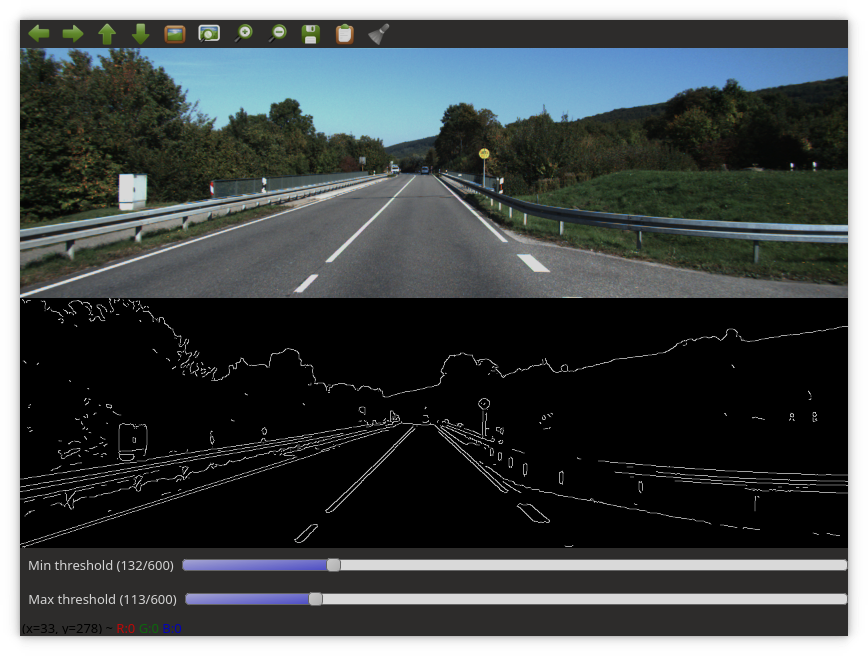
\includegraphics[width=0.9\textwidth]{./canny_demo.png}
                \end{center}
                It is possible to tune two paramters:
                \begin{itemize}
                    \item $Min\ Threshold$: this acts as a sort of erosion on the
                        edges: when you raise this parameter you cancel out
                        weak part of edges connected with stronger
                        ones
                    \item $Max\ Threshold$: this acts like a real threshold on
                        edges because it deletes entire edges based on their
                        strength, so if an edge became non so strong (by setting
                        an higher threshold) also the weak parts of that edge (which 
                        falls between the two thresholds) are deleted
                \end{itemize}
                Implementation don't check if $Min\ Threshold\ \le\
                Max\ Threshold$ because it is possible to obtain interesting
                results. Usually the higher threshold is three times the lower
                one. 
            \item Last step is to apply Hough Lines Transform on the Canny
                image:
                \begin{center}
                    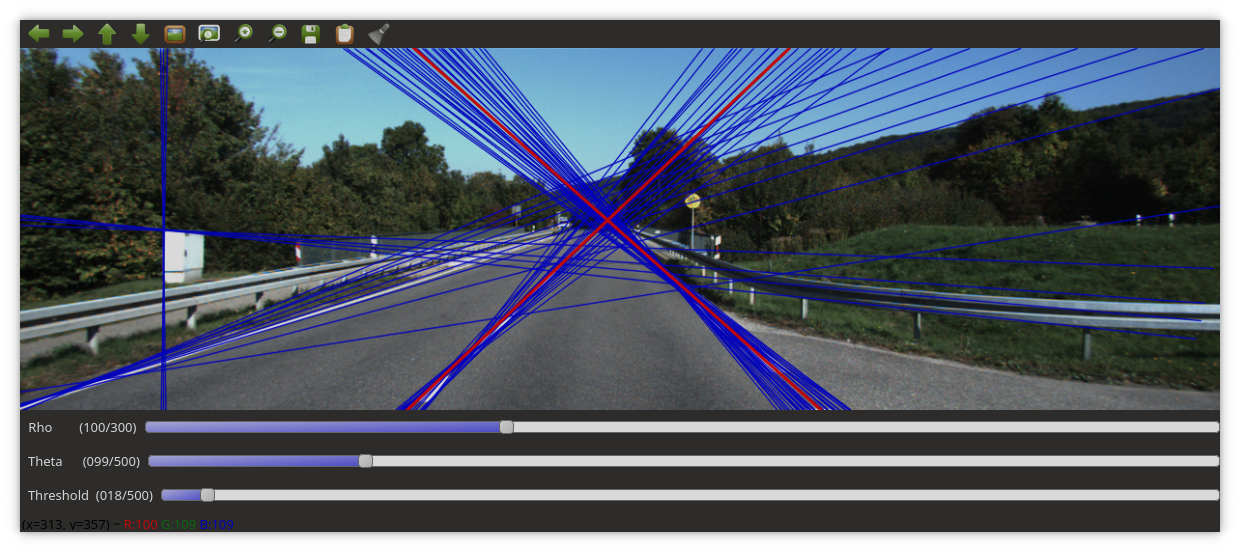
\includegraphics[width=0.9\textwidth]{./lines_demo.png}
                \end{center}
                The blue lines are detected lines, the red ones is the ones with
                more score. It is possible to tune three paramters:
                \begin{itemize}
                    \item $Rho$: resolution of $\rho$ in pixel. Usually it is
                        left as 1.0, but with small changes it is possible to
                        select the desidered lines.
                    \item $Theta$: resolution of $\theta$ in degree. Usually it
                        is left as 1 degree but, as $Rho$, it is possible to
                        select different lines by small changes (like switch
                        between the guard rail and the asphalt lines).
                    \item $Threshold$
                \end{itemize}
        \end{enumerate}
    \item Circles detection: performed in one shot because the OpenCV method
        also contain the Canny edges detection:
            \begin{center}
                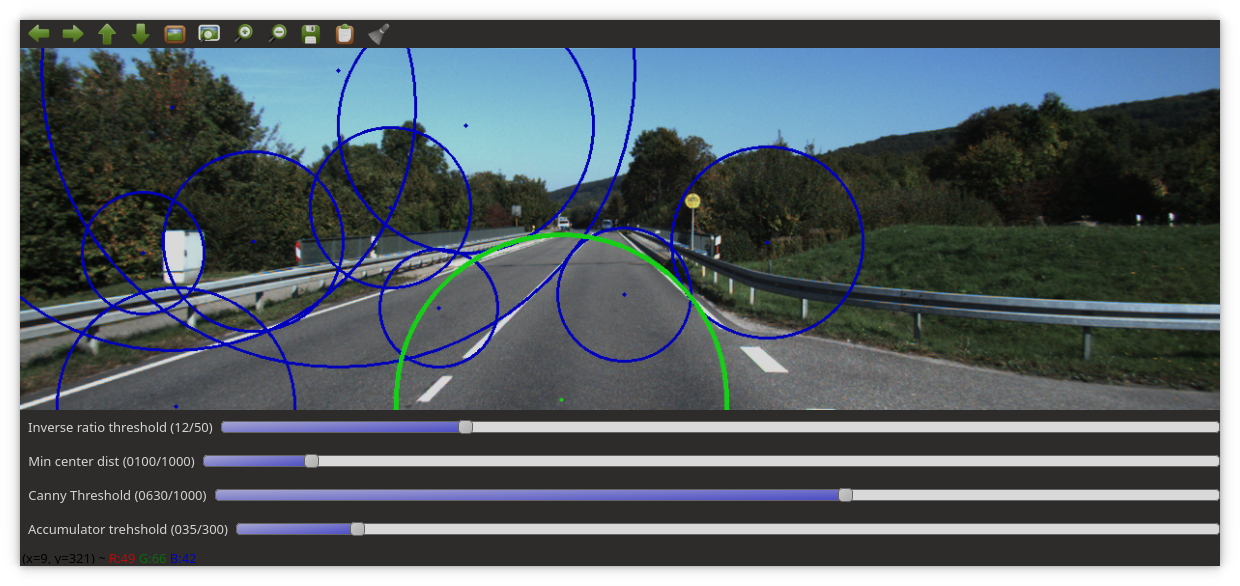
\includegraphics[width=0.9\textwidth]{./circles_demo.png}
            \end{center}
        The tunable parameters are four:
        \begin{itemize}
            \item $Inverse\ ratio\ threshold$: since the selected method for
                detection is \mintinline{R}{HOUGH_GRADIENT} this parameter should 
                remain in range between 1.0 and 1.5
            \item $Minimum\ dist\ between\ centers$: minimum distance between
                circles centes such that they are both detected: userful to
                filter out lots of small circles 
            \item $Canny\ threshold$: max threshold during Canny edges
                detection, the min threshold is computed as half of this one.
                This parameter is very important since, fixed the previous two
                ones, it makes possible to perform a good detection. (As a Canny
                does previously with lines detection.) The idea is
                to find a good threhsold in step 1a and report the value here.
            \item $Accumulator\ threshold$
        \end{itemize}
        With some combination of values (in particular small value on the last
        three parametrs) it is possible to detect thousand of circles, creating
        computational issues.
    \item The last part is about retrive the information of lines and circles
        and draw on screen the detected part. The final result is this one:
            \begin{center}
                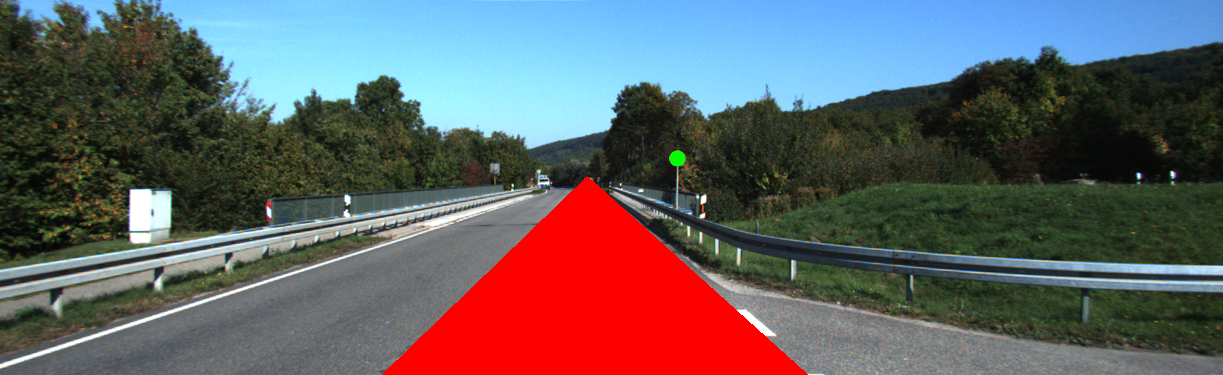
\includegraphics[width=0.9\textwidth]{./final.png}
            \end{center}
\end{enumerate}
Note: all the parameters are pre-tuned in order to perform the better result.


\end{document}
